\documentclass[a4paper,10pt]{article}

\usepackage{hyperref}
\usepackage{mathpazo}
\usepackage{amsmath}

\usepackage{tikz}
\usetikzlibrary{calc}

\setlength{\oddsidemargin}{-0.4mm}    % 25 mm left margin - 1 in
\setlength{\evensidemargin}{\oddsidemargin}
\setlength{\topmargin}{-5.4mm}        % 20 mm top margin - 1 in
\setlength{\textwidth}{160mm}         % 20/25 mm right margin
\setlength{\textheight}{247mm}        % 20 mm bottom margin
\setlength{\headheight}{5.1mm}
\setlength{\headsep}{5mm}
\setlength{\parindent}{0mm}
\setlength{\parskip}{\medskipamount}

\title{0 A.D.\@ Pathfinder Design}
\author{Wildfire Games -- \url{http://wildfiregames.com/}}

\begin{document}

\maketitle

\tableofcontents

\section{Basic concepts}

Our world consists of:
\begin{itemize}
 \item \textbf{Units} --
  Small, mobile objects.
  Units move along the ground (or water, if they're ships).
  They have instant acceleration and deceleration, and zero turning circles.
 \item \textbf{Structures} --
  Possibly-large, stationary objects.
  This includes buildings, walls, trees, rocks, etc.
 \item \textbf{Terrain} --
  2D grid with a heightmap and other per-terrain-tile data (e.g.\ texture),
  plus a water plane.
\end{itemize}

Units and structures are not restricted to terrain tiles in any way --
they can have high-precision positions and can face in any direction.
Both are represented as \emph{obstruction squares} -- we simplify their shapes to
a single square\footnote{For ``square'', read ``rectangle''. Or ``affine transformation of a square'' if you prefer.}.
Units are typically humanoids and should move in at least roughly human-like ways
(not e.g.\ like hover-tanks).
Units should never move through structures,
and in general should never move through other units (except in special cases like formations).

The world might have something like 1000 units (all moving at once),
$256\times256$ terrain tiles, 100 buildings, 1000 trees.
The target platform is PCs (in particular x86 or x86\_64 with 512+ MB RAM;
we can use a lot of memory for pathfinding if necessary).

\emph{Pathfinding} is the operation of picking a route for a unit to move along
from its current location to any other location in the world,
so that it does not collide with other units
or with structures or with impassable terrain.
The picked route should be the shortest (or an equal shortest) of all possible routes.

Pathfinding is split into two levels.
The \emph{long-range pathfinder} is responsible for finding approximate routes
that can span from one corner of the map to the other.
It only needs to care about structures and terrain;
any units in the way will probably have moved by the time the pathing unit reaches them,
so there's no need for the long-range pathfinder to plan around them.
It can approximate the world as a 2D grid.
The \emph{short-range pathfinder} is responsible for computing precise paths
that follow a segment of the long-range path --
these should not be quantised to a grid (since that would look ugly),
and should avoid other units,
but only need to work over a short distance (to the next waypoint on the long-range path).

\subsection{Coordinates}

Units have an $(x, z)$ position, measured in `metres' (the generic world-space unit of distance).
The coordinates are implemented as fixed-point numbers
(with a 16-bit fraction, i.e.\ a resolution of $2^{-16}\mathrm{m} \approx 15\mu\mathrm{m}$),
but we can treat them as real numbers.
The positive $x$ direction is interpreted as right or east; the positive $z$ direction is up or north.

\emph{Navcells} (the tile-like concept used for navigation)
are squares identified as $(i, j)$,
corresponding to world-space coordinates
\begin{align*}
i \times \mathrm{NavcellSize} & \leq x < (i+1) \times \mathrm{NavcellSize} \\
j \times \mathrm{NavcellSize} & \leq z < (j+1) \times \mathrm{NavcellSize}
\end{align*}
where $\mathrm{NavcellSize}$ is typically $1.0$ in the current implementation.

A unit is always located on a single navcell:
\[
\mathrm{PointToNavcell}(x, z) = (\lfloor x / \mathrm{NavcellSize} \rfloor, \lfloor z / \mathrm{NavcellSize} \rfloor)
\]

\subsection{Units}

Units have a \emph{unit obstruction} shape,
with a defined radius.
The shape is usually interpreted as an axis-aligned square
(with width and height equal to $2\times\mathrm{UnitRadius}$),
but sometimes interpreted more like a circle.
Infantry units might have a radius of around 0.5,
while siege units might have a radius of around 4.

Units also have a passability class,
which defines various details about what kinds of terrain they can cross.
Most of the data structures used by the pathfinder are
duplicated once per passability class.
For this document, we'll mostly just describe algorithms in terms of a single passability class,
and the implementation implicitly picks the appropriate data for the current unit's class.

There might be something like 8--16 distinct passability classes in the game.

Passability classes also define a \emph{clearance} value,
which is typically similar to their obstruction radius,
defining how close they can get to structures or impassable terrain.
Clearance should be a multiple of $\mathrm{NavcellSize}$.

TODO: Constraints on clearance vs radius?

\subsection{Structures}

Structures are represented by \emph{static obstruction squares},
which are non-axis-aligned parallelograms
defined by $(x, z, \frac{w}{2}, \frac{h}{2}, \mathbf{u}, \mathbf{v})$:

\begin{tikzpicture}[>=stealth,scale=0.5]

\node (o) at (0,0) [label=below:{$(x,z)$}] {};
\draw (0,0) circle (0.1cm);
\node (a) at (3,4) [label=above:{$(x,z) + \frac{w}{2}\mathbf{u} + \frac{h}{2}\mathbf{v}$}] {};
\node (b) at (5,0) [label=right:{$(x,z) + \frac{w}{2}\mathbf{u} - \frac{h}{2}\mathbf{v}$}] {};
\node (c) at (-3,-4) [label=below:{$(x,z) - \frac{w}{2}\mathbf{u} - \frac{h}{2}\mathbf{v}$}] {};
\node (d) at (-5,0) [label=left:{$(x,z) - \frac{w}{2}\mathbf{u} + \frac{h}{2}\mathbf{v}$}] {};

\draw[<->,dashed] (o) -- (4,2) node[below,midway] {$\frac{w}{2}$};
\draw[<->,dashed] (o) -- (-1,2) node[left,midway] {$\frac{h}{2}$};

\draw
  (3,4) circle (0.1cm) --
  (5,0) circle (0.1cm) --
  (-3,-4) circle (0.1cm) --
  (-5,0) circle (0.1cm) --
  (3,4);

\begin{scope}[xshift=-6cm,yshift=-3cm]
\draw[->] (0,0) -- (1,0.5) node[right] {$\mathbf{u}$};
\draw[->] (0,0) -- (-0.5,1) node[above] {$\mathbf{v}$};
\end{scope}

\end{tikzpicture}

The $\mathbf{u}$ and $\mathbf{v}$ are unit vectors.
They should be perpendicular; that's not theoretically required,
but some of the implementation assumes that.

We actually store the half-width $\frac{w}{2}$ (as ``\texttt{hw}'' in the code)
instead of $w$, because that seems more convenient for the implementation.
(Same for $h$.)

We store $\mathbf{u}$ and $\frac{w}{2}$ as two values,
instead of premultiplying them and using a single (non-unit) vector everywhere,
because occasionally we really need the unit vectors (e.g.\ to compute
world-space distance from a point to a square).

Some of the game code uses a representation $(x, z, w, h, \theta)$ instead
(where $\theta$ is anticlockwise from the $x$ axis),
which is more convenient for editing.
That is transformed into the vector form
(which is more convenient for geometric computation)
for the purposes of the algorithms described in this document.

\section{Navcell grid}

The long-range pathfinder can be simpler and more efficient if it has a
grid representation of the map.
(Since our maps are large and open (i.e.\ a high degree of connectivity
between areas), and must support dynamic generation (random map scripts)
and dynamic modification (new buildings, walls, etc),
a grid is likely better than a nav mesh.)

Terrain is already based on a grid representation of the map,
but it is pretty low resolution (tiles have size $4.0 \times 4.0$;
you could fit 16 units onto a single terrain tile without much trouble)
so it will be poor at approximating narrow gaps which a single unit could fit through.
Increasing the terrain resolution would mean more heightmap and texture-pointer data
(10 bytes per tile),
more graphics data
(at least 16 bytes per tile, more when blending between textures),
and more triangles to render per frame.
It's better if we can use a higher-resolution grid for pathfinding than for terrain.

Pathfinding therefore uses a navcell grid, independent of the terrain grid.
Navcell passability is encoded as a 2D array covering the map,
with one bit per passability class.
Passability is computed from terrain and from static obstructions.

\subsection{Terrain}

(Implemented by \texttt{CCmpPathfinder::UpdateGrid}.)

A passability class defines maximum terrain slope, min/max water depth, etc.
For each navcell, we compute slopes and depths from the terrain heightmap.
When navcells are higher resolution than the heightmap, we do some interpolation
to get smoother output.

That will give a binary \emph{terrain passability grid} for this passability class:

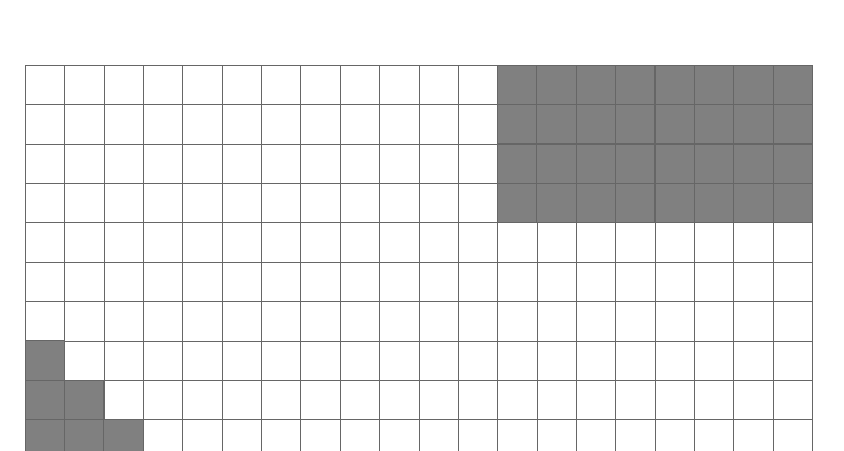
\begin{tikzpicture}[
  scale=0.5,
  blocked/.style={rectangle,draw=black!60,fill=black!50,minimum size=0.5cm}
]

\draw[step=1cm,black!60,very thin,xshift=-0.5cm,yshift=-0.5cm] (0,0) grid (20,10);

\foreach \x in {0,1,2} \node[blocked] at (\x,0) {};
\foreach \x in {0,1} \node[blocked] at (\x,1) {};
\foreach \x in {0} \node[blocked] at (\x,2) {};
\foreach \x in {12,...,19}
  \foreach \y in {6,7,8,9}
    \node[blocked] at (\x,\y) {};

\end{tikzpicture}

We also force the navcells around the outside of the map to be impassable.
(This means we usually don't have to worry about units walking off the edge of the map.
It also means we can use the shroud-of-darkness effect to make the map smoothly fade out
around its edges, and units won't walk so far out that they disappear into that SoD.\@)
This is either a circular or square pattern,
and we currently have at least 3 impassable terrain tiles (i.e.\ currently 12 navcells)
around each edge.

The grid is then expanded by the passability class's clearance value $c$
(effectively convolution with a square filter of size $(2c+1)\times(2c+1)$)
to get the \emph{expanded terrain passability grid}:

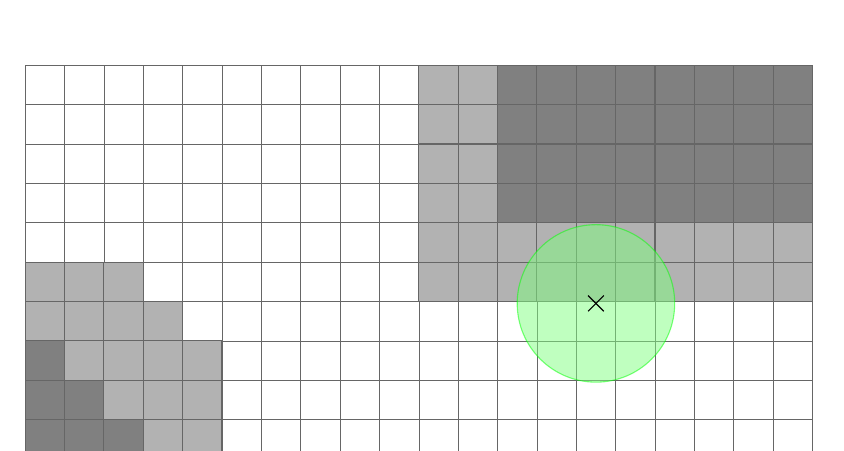
\begin{tikzpicture}[
  blocked/.style={rectangle,draw=black!60,fill=black!50,minimum size=0.5cm},
  blocked2/.style={rectangle,draw=black!60,fill=black!30,minimum size=0.5cm},
  scale=0.5
]

\def\unit#1;{
  \draw[draw=green,fill=green!50,opacity=0.5] #1 circle (2cm);
  \draw[draw=black] #1 ++(-0.2cm,-0.2cm) -- ++(0.4cm,0.4cm);
  \draw[draw=black] #1 ++(-0.2cm,0.2cm) -- ++(0.4cm,-0.4cm);
}

\draw[step=1cm,black!60,very thin,xshift=-0.5cm,yshift=-0.5cm] (0,0) grid (20,10);

\node[blocked] at (0,0) {};
\node[blocked] at (1,0) {};
\node[blocked] at (2,0) {};
\node[blocked] at (0,1) {};
\node[blocked] at (1,1) {};
\node[blocked] at (0,2) {};

\foreach \x in {0,1,2} \node[blocked] at (\x,0) {};
\foreach \x in {0,1} \node[blocked] at (\x,1) {};
\foreach \x in {0} \node[blocked] at (\x,2) {};
\foreach \x in {12,...,19}
  \foreach \y in {6,7,8,9}
    \node[blocked] at (\x,\y) {};

\foreach \x in {3,4} \node[blocked2] at (\x,0) {};
\foreach \x in {2,3,4} \node[blocked2] at (\x,1) {};
\foreach \x in {1,2,3,4} \node[blocked2] at (\x,2) {};
\foreach \x in {0,1,2,3} \node[blocked2] at (\x,3) {};
\foreach \x in {0,1,2} \node[blocked2] at (\x,4) {};

\foreach \x in {10,11}
  \foreach \y in {6,7,8,9}
    \node[blocked2] at (\x,\y) {};

\foreach \x in {10,...,19}
  \foreach \y in {4,5}
    \node[blocked2] at (\x,\y) {};

\unit (14,3.45);

\end{tikzpicture}

(It'd be nicer to do a more circular convolution, so that the sharp corner
in the top-right gets smoothed to a more rounded corner,
especially with large clearance values.
That would be a self-contained enhancement and won't have any further consequences.)

A unit may be located anywhere on any passable navcell in this new grid.
If a unit is visualised as a circle with radius $r$,
then the circle won't overlap any impassable navcell in the
original terrain passability grid as long as $c \geq r$.
The green circle in the previous figure indicates a unit with $r=2$
in a valid location.

\subsection{Static obstructions}

(Implemented by \texttt{CCmpObstructionManager::Rasterize}.)

Rasterization is the process of converting a vector shape
(in this case an obstruction square)
into a pixel grid (in this case actually a navcell grid).
We do this so that the grid-based pathfinders can handle static obstructions (like walls)
in the same way as they handle terrain-based obstructions (like rivers).

For a given clearance value $c$,
a navcell is blocked by an obstruction shape
if every corner of the navcell
is either inside the shape or is a distance $d \leq c$ away from the shape.

In the following figure, blue is obstruction squares, red is the points at distance $c=1$
outside of the obstruction square,
green circles are some units with radius 1,
and grey squares are blocked by the obstructions.

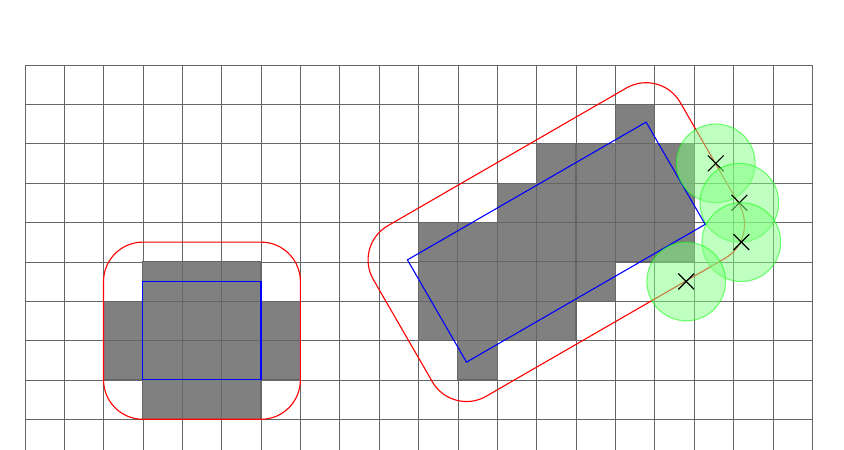
\begin{tikzpicture}[
  scale=0.5,
  blocked/.style={rectangle,draw=black!60,fill=black!50,minimum size=0.5cm}
]

\def\unit#1;{
  \draw[draw=green,fill=green!50,opacity=0.5] #1 circle (1cm);
  \draw[draw=black] #1 ++(-0.2cm,-0.2cm) -- ++(0.4cm,0.4cm);
  \draw[draw=black] #1 ++(-0.2cm,0.2cm) -- ++(0.4cm,-0.4cm);
}

\draw[step=1cm,black!60,very thin,xshift=-0.5cm,yshift=-0.5cm] (0,0) grid (20,10);

\begin{scope}[xshift=4cm,yshift=3cm]
\foreach \x in {-1,...,1} \node[blocked] at (\x,-2) {};
\foreach \x in {-2,...,2} \node[blocked] at (\x,-1) {};
\foreach \x in {-2,...,2} \node[blocked] at (\x,0) {};
\foreach \x in {-1,...,1} \node[blocked] at (\x,1) {};
\draw [color=red,rounded corners=0.5cm] (-2.5,-2.5) rectangle (2.5,2);
\draw [color=blue] (-1.5,-1.5) rectangle (1.5,1);
\end{scope}

\begin{scope}[xshift=13cm,yshift=5cm]
\foreach \x in {2} \node[blocked] at (\x,3) {};
\foreach \x in {0,...,3} \node[blocked] at (\x,2) {};
\foreach \x in {-1,...,3} \node[blocked] at (\x,1) {};
\foreach \x in {-3,...,3} \node[blocked] at (\x,0) {};
\foreach \x in {-3,...,1} \node[blocked] at (\x,-1) {};
\foreach \x in {-3,...,-0} \node[blocked] at (\x,-2) {};
\foreach \x in {-2} \node[blocked] at (\x,-3) {};
\draw [color=red,rotate=30,rounded corners=0.5cm] (-4.5,-2.5) rectangle (4.5,2.5);
\draw [color=blue,rotate=30] (-3.5,-1.5) rectangle (3.5,1.5);

\unit (4.05,2);
\unit (4.65,1);
\unit (4.7,0);
\unit (3.3,-1);

\end{scope}

\end{tikzpicture}

It is important that partially-obstructed navcells are still considered passable:
when a unit is trying to move to a building (e.g.\ to attack it),
it can always succesfully get within any distance $d > c$ of the obstruction shape,
without having to move illegally onto an impassable navcell.

TODO: In the implementation, we need to be sure units never try to move
within a distance $d \leq c$, else they might be blocked by navcells.
Maybe add $c$ to all (positive) attack/gather/etc ranges?

\subsection{Narrow obstructions}

If an obstruction is especially narrow (e.g.\ a fence),
it might not block any navcells and units could walk straight through it,
which would surprise map designers.

The worst case is when rotated 45 degrees,
in which a long obstruction
must be at least $\frac{3}{\sqrt{2}}$ (about 2.12) navcells wide
(including the clearance expansion),
and a square obstruction must be at least $2\sqrt{2}$ (about 2.83) wide:

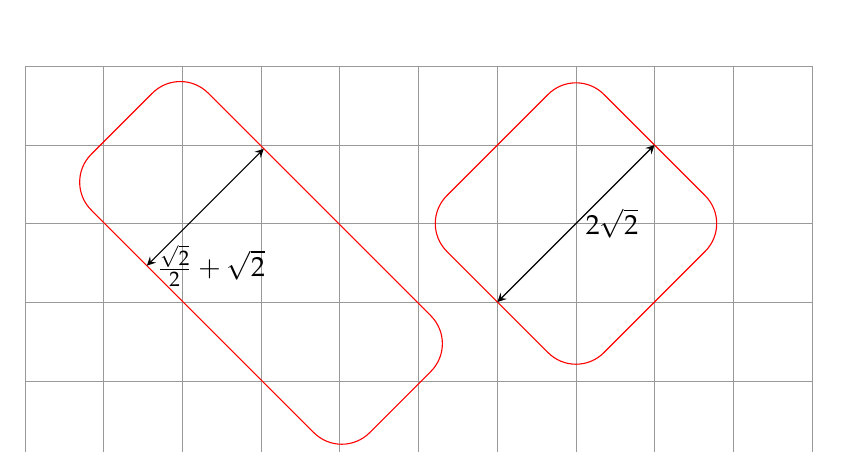
\begin{tikzpicture}[
  >=stealth,
  blocked/.style={rectangle,draw=black!60,fill=black!50,minimum size=0.5cm}
]

\draw[step=1cm,black!40,very thin,xshift=-0.5cm,yshift=-0.5cm] (0,0) grid (10,5);

\begin{scope}[xshift=2.5cm,yshift=2cm]
\draw [color=red,rotate=45,rounded corners=0.5cm] (-1.05,-2.5) rectangle (1.05,2.5);
\draw[<->,rotate=45] (-1.05,1) node[right] {$\frac{\sqrt{2}}{2}+\sqrt{2}$} -- (1.05,1) ;
\end{scope}

\begin{scope}[xshift=6.5cm,yshift=2.5cm]
\draw [color=red,rotate=45,rounded corners=0.5cm] (-1.41,-1.41) rectangle (1.41,1.41);
\draw[<->,rotate=45] (-1.41,0) -- (1.41,0) node[midway,right] {$2\sqrt{2}$} ;
\end{scope}

\end{tikzpicture}

But there are still problems when a long obstruction is $\sqrt{5}$ (about 2.24) wide,
since it may contain gaps that units can walk through:

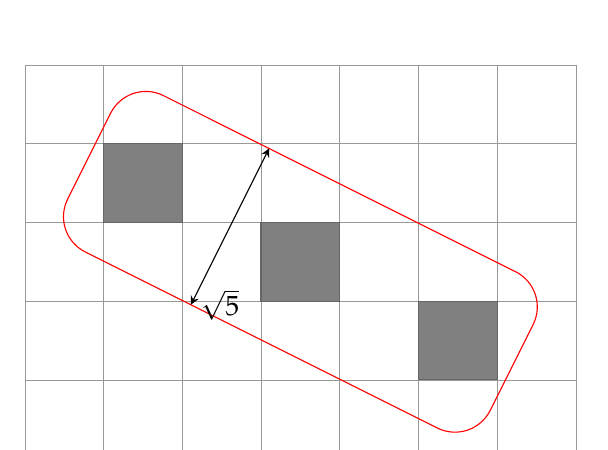
\begin{tikzpicture}[
  >=stealth,
  blocked/.style={rectangle,draw=black!60,fill=black!50,minimum size=1cm}
]

\draw[step=1cm,black!40,very thin,xshift=-0.5cm,yshift=-0.5cm] (0,0) grid (7,5);

\begin{scope}[xshift=3cm,yshift=2cm]
\draw [color=red,rotate=63.43,rounded corners=0.5cm] (-1.11,-3) rectangle (1.11,3);
\draw[<->,rotate=63.43] (-1.11,1) node[right] {$\sqrt{5}$} -- (1.11,1) ;
\node[blocked] at (-2,1) {};
\node[blocked] at (0,0) {};
\node[blocked] at (2,-1) {};
\end{scope}

\end{tikzpicture}

To avoid these problems,
when rasterizing a rectangle of size $(w,h)$ with clearance $c$,
we will instead rasterize a rectangle of size $(w,h)$ with clearance $\max(c,\ (3-\min(w,h))/2)$
(where 3 is a nice round number that's definitely bigger than the limits demonstrated here).
When the smallest unit has $c=1$,
that limit will only take effect for obstructions with $w < 1$ or $h < 1$.

\section{Path goals}

When a path is requested, there is a source unit and a goal.
The goal might be:
\begin{itemize}
 \item Point $(x, z)$ --
 e.g.\ when telling a unit to walk to some specific location.
 \item Square $(x, z, \frac{w}{2}, \frac{h}{2}, \mathbf{u}, \mathbf{v})$ --
 e.g.\ when telling
 a melee unit to attack a square building, they will move to positions close to the building
 (depending on their maximum attack range) in a square pattern.
 \item Circle $(x, z, r)$ --
 e.g.\ when telling
 a ranged unit to attack a square building, they will move to positions within
 maximum attack range of the building in a circular pattern.
 \item TODO: Inverted squares/circles for minimum attack range?
\end{itemize}

TODO: Need some constraints on squares/circles that are based on structures,
so they're always far enough out.

A navcell can be considered to be \emph{inside a goal}.
If the goal is a point $(x, z)$, then only the navcell $\mathrm{PointToNavcell}(x, z)$
is inside the goal.
Otherwise, a navcell is inside the goal if any point inside (or on the edge of) that navcell
is inside (or on the edge of) the goal shape.

TODO: Think about edges cases in relation to vertex pathfinder.

\section{Navcell-based A* pathfinder}

The basic pathfinder is a pretty standard A* over a uniform-cost grid of navcells.
Connectivity between navcells is as illustrated:

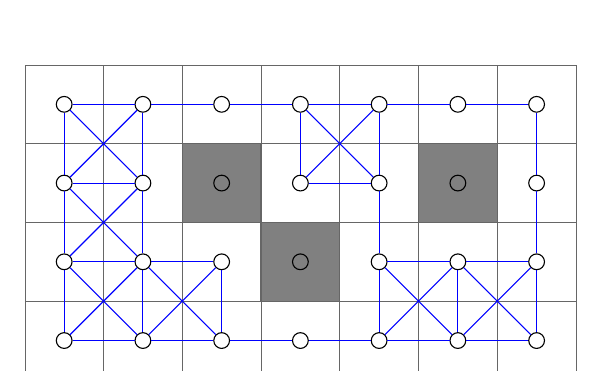
\begin{tikzpicture}[
  blocked/.style={rectangle,draw=black!60,fill=black!50,minimum size=1cm}
]

\def\unit#1;{
  \draw[draw=green,fill=green!50,opacity=0.5] #1 circle (1cm);
  \draw[draw=black] #1 ++(-0.2cm,-0.2cm) -- ++(0.4cm,0.4cm);
  \draw[draw=black] #1 ++(-0.2cm,0.2cm) -- ++(0.4cm,-0.4cm);
}

\draw[step=1cm,black!60,very thin,xshift=-0.5cm,yshift=-0.5cm] (0,0) grid (7,4);

\node[blocked] at (2,2) {};
\node[blocked] at (3,1) {};
\node[blocked] at (5,2) {};

\foreach \x in {0,...,6}
  \foreach \y in {0,...,3}
    \draw (\x,\y) circle (0.1cm) node [circle,inner sep=0.07cm] (c\x\y) {};

\begin{scope}[color=blue]
\draw (c03)--(c13)--(c23)--(c33)--(c43)--(c53)--(c63);
\draw (c02)--(c12); \draw (c32)--(c42);
\draw (c01)--(c11)--(c21); \draw (c41)--(c51)--(c61);
\draw (c00)--(c10)--(c20)--(c30)--(c40)--(c50)--(c60);
\draw (c03)--(c02)--(c01)--(c00);
\draw (c13)--(c12)--(c11)--(c10);
\draw (c21)--(c20);
\draw (c33)--(c32);
\draw (c43)--(c42)--(c41)--(c40);
\draw (c51)--(c50);
\draw (c63)--(c62)--(c61)--(c60);

\draw (c03)--(c12)--(c01)--(c10);
\draw (c13)--(c02)--(c11)--(c00);
\draw (c11)--(c20);
\draw (c21)--(c10);
\draw (c33)--(c42);
\draw (c43)--(c32);
\draw (c40)--(c51)--(c60);
\draw (c41)--(c50)--(c61);
\end{scope}

\end{tikzpicture}

From any passable navcell, you can move to any horizontally/vertically adjacent
passable navcell with cost $1$.
Also, you can move diagonally from any navcell $(i,j)$ to $(i\pm1,j\pm1)$
if those navcells,
plus the adjacent navcells $(i\pm1,j\mp1)$ and $(i\mp1,j\pm1)$,
are all passable.
Diagonal moves have cost $\sqrt{2}$.

Note that this definition of diagonal movement
means that connectivity between any two navcells
can be determined solely from the horizontal/vertical adjacencies;
the only effect of the diagonal moves is to allow smoother shorter paths.

\section{JPS A* pathfinder}

This is just an optimisation of standard navcell-based A*,
which works especially well on sparse grids.

TODO: Details.

\section{Hierarchical pathfinder}

This can do the following:
\begin{itemize}
 \item Determine if there is at least one path through the navcell grid between
 passable navcells $a$ and $b$ (i.e.\ determine if $b$ is \emph{reachable} from $a$).
 \item Given a goal shape and a passable source navcell $a$,
 determine if there is any navcell that is in the goal and is reachable from $a$.
 If not, find one of the reachable navcells that is nearest to the center of the goal.
 \item Given an impassable navcell $a$, find one of the passable navcells that is
 nearest to $a$.
\end{itemize}

Note that it doesn't actually find paths.
We might want to extend it to do that in the future,
if JPS is too slow.

TODO: Details.

\section{Vector pathfinder}

In addition to the navcell-based pathfinders (which are fine for approximate paths
over a fairly static grid with large obstructions,
but not good at fine detail or at very frequent changing or small obstructions),
we have a pathfinder based on a vector representation of the world.

The current implementation is a points-of-visibility pathfinder.
The world is represented as a set of edges (impassable straight lines for the outlines of obstructions)
and a set of vertexes (for the corners of obstructions).
Edges are single-sided (they block movement from outside an obstruction to the inside,
but not vice versa).
A path can go from any vertex to any other vertex, if the straight line between those vertexes
does not intersect any obstruction edges.
Given those vertexes and connectivity data,
a basic implementation of A* can find optimal paths.

The vector pathfinder has to understand terrain-based impassability
(which is fundamentally defined on a navcell grid),
static obstructions, and dynamic obstructions.
(Dynamic obstructions are other units -- they are smallish,
and can be treated as circles or axis-aligned squares or similar.)

Inconsistencies between the navcell pathfinder and vector pathfinder are problematic.
If the navcell pathfinder thinks a route is blocked,
but the vector pathfinder thinks there is enough space,
then units will sometimes use that route and sometimes refuse to.
In the opposite case, the navcell pathfinder will send a unit along a route
that it thinks is valid,
but the vector pathfinder will think there's not actually enough space
and the unit will be stuck and won't know where to go.
This is inevitable when a route is blocked by dynamic obstructions,
but we should aim to avoid such problems in at least the cases where there are
no dynamic obstructions.

To minimise those inconsistencies,
the vector pathfinder uses the navcell-grid rasterized versions of static obstructions,
instead of using the original rotated-rectangle vector versions.

The pathfinder algorithm does not explicitly take account of the unit's size --
it assumes the unit is a point and can move arbitrarily close to an obstruction edge.
Because the navcell grid has already encoded the unit's clearance value,
we can convert the navcell outlines directly into the vector representation
for this pathfinder, and units will not get too close to static obstructions.

Note that since navcells intersecting the edge of a static obstruction
are not made impassable,
the vector pathfinder will let units move slightly inside the
geometric shape of the obstruction
(by up to $\sqrt{2}\times\mathrm{NavcellSize}$).
(TODO: Be more specific/correct.)

Dynamic obstructions (units etc) are converted directly into vectors,
without quantising to the navcell grid.
Their obstruction shapes are axis-aligned squares with a known radius.
To stop units intersecting each other,
each square is expanded by the pathing unit's own obstruction radius.

Note that all edges (from dynamic obstructions and from the navcell grid)
are axis-aligned. This allows some simplifications and optimisations,
and avoids precision issues when deciding whether a point is precisely on a line.

TODO: Inconsistency between clearance and obstruction radius?

The pathfinder can then find paths between corners that don't intersect edges.

TODO: How does it handle edge cases like units starting precisely on an edge?

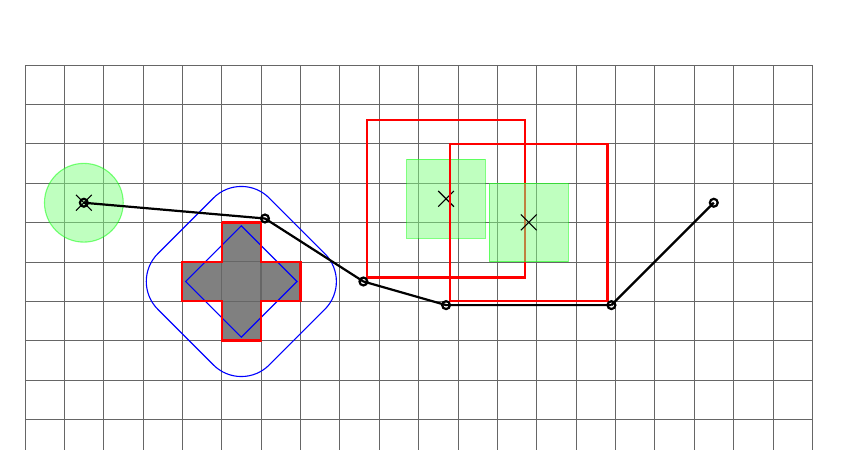
\begin{tikzpicture}[
  >=stealth,
  scale=0.5,
  blocked/.style={rectangle,draw=black!60,fill=black!50,minimum size=0.5cm}
]

\def\unit#1;{
  \draw[draw=green,fill=green!50,opacity=0.5] #1 circle (1cm);
  \draw[draw=black] #1 ++(-0.2cm,-0.2cm) -- ++(0.4cm,0.4cm);
  \draw[draw=black] #1 ++(-0.2cm,0.2cm) -- ++(0.4cm,-0.4cm);
}

\def\unitb#1;{
  \draw[draw=red,thick] ($#1-(2cm,2cm)$) rectangle ($#1+(2cm,2cm)$);
  \draw[draw=green,fill=green!50,opacity=0.5] ($#1-(1cm,1cm)$) rectangle ($#1+(1cm,1cm)$);
  \draw[draw=black] #1 ++(-0.2cm,-0.2cm) -- ++(0.4cm,0.4cm);
  \draw[draw=black] #1 ++(-0.2cm,0.2cm) -- ++(0.4cm,-0.4cm);
}

\draw[step=1cm,black!60,very thin,xshift=-0.5cm,yshift=-0.5cm] (0,0) grid (20,10);

\begin{scope}[xshift=5cm,yshift=4cm]

\foreach \x in {0} \node[blocked] at (\x,1) {};
\foreach \x in {-1,0,1} \node[blocked] at (\x,0) {};
\foreach \x in {0} \node[blocked] at (\x,-1) {};
\draw [color=blue,rounded corners=0.5cm,rotate=45] (-2,-2) rectangle (2,2);
\draw [color=blue,rotate=45] (-1,-1) rectangle (1,1);

\draw [color=red,thick] (-0.5,1.5) -- ++(1,0) -- ++(0,-1) -- ++(1,0) -- ++(0,-1) -- ++(-1,0) -- ++(0,-1) -- ++(-1,0)
 -- ++(0,1) -- ++(-1,0) -- ++(0,1) -- ++(1,0) -- ++(0,1);

\unitb (5.2,2.1);
\unitb (7.3,1.5);

\unit (-4,2);
\draw [color=black,thick]
  (-4,2) circle (0.1cm) --
  (0.6,1.6) circle (0.1cm) --
  (3.1,0.0) circle (0.1cm) --
  (5.2,-0.6) circle (0.1cm) --
  (9.4,-0.6) circle (0.1cm) --
  (12,2) circle (0.1cm);

\end{scope}

\end{tikzpicture}

\section{Stuck units}

(Implemented by \texttt{CCmpPathfinder::ComputePathOffImpassable}.)

A unit might find itself on an impassable navcell.
(We should prevent that whenever possible,
but we should be robust to error cases where the prevention fails,
and it can easily happen in Atlas.)
The JPS pathfinder and hierarchical goal reachability system
inherently require that units start on passable navcells.
We therefore need a way to safely get units off impassable navcells as quickly as possible.

The hierarchical pathfinder can find the nearest passable navcell to the unit.
We can then construct a straight-line path to that navcell,
and let the unit recompute a proper path once it's got out.

Normally the short-range pathfinder will let the unit get quite widely diverted from the long-range path.
That's bad when the unit is starting inside a building or a region of impassable terrain --
it might decide to go a very long way through the impassable region,
instead of getting out as quickly as possible.

TODO: How can we handle that? (Add a flag to disable the short-range pathfinder?
What if another unit is in the way?)

\section{Minimum ranges}

Some units have a minimum attack range (e.g.\ a ballista can't be aimed
at someone standing right in front of it).
If they are too close to their target,
they need to move away from it before being able to attack.

Minimum ranges will usually be quite small -- maybe 16 navcells at most.
That's short enough that the short-range pathfinder will always suffice;
we don't need to use the long-range pathfinder to work out how to move
away from the target.
This means the long-range pathfinder only has to care about how to move
towards a target (which avoids some minor complexities in the implementation).

The short-range pathfinder already moves to the edge of a goal shape,
and doesn't care whether the unit is starting inside or outside that shape.
That means it'll work for minimum-range movement with no futher modifications.

\section{Unit movement}

The short-range pathfinder will give the unit a waypoint to walk towards.
The unit will move a short distance in that direction each turn.
To cope with dynamic changes to the world,
the unit needs to verify that its movement won't collide with anything.
This requires testing the movement line against the navcell grid,
and against unit obstructions (expanded by the moving unit's radius).
If there is a collision then the unit won't move, and will search for
a new path instead.

TODO: Does the implementation work like that?

To check collisions with other units,
we expand every unit obstruction shape by the moving unit's radius,
and test the movement line against those squares.
TODO: How is the testing done, precisely?
If the start point is inside (or on the edge of) the square,
then it will never collide;
otherwise, if the end point is inside (or on the edge)
then it collides;
otherwise, it tests whether the line passes through the square
(TODO: edge cases).

This means a unit must never be placed precisely on the edge
of another unit obstruction -- it will be able to move inside the second unit.
If a unit is not inside (or on the edge),
it will never be able to move so that is inside (or on the edge),
so we just need to be careful when spawning new units to avoid starting too close.

TODO: Describe the navcell passability testing.

\section{Unit spawning}

(Implemented by \texttt{CCmpFootprint::PickSpawnPoint}
and \texttt{CCmpPathfinder::CheckUnitPlacement}.)

When a building trains a unit, it needs to pick positions nicely located
around the perimeter for the units to appear.
(We don't have units walking out of a door, they just appear instantly.)
A position is valid if it is on a passable navcell,
and if the unit doesn't overlap with any existing units.

TODO: The implementation tests against static obstructions unnecessarily.

\section{Building placement}

(Implemented by \texttt{CCmpObstruction::CheckFoundation}
and \texttt{CCmpPathfinder::CheckBuildingPlacement}.)

Buildings have various terrain restrictions (maximum slope,
min/max water depth, distance from shore, etc)
defined as a passability class.
Players should only be permitted to place a building if every navcell
under the building is valid,
so that they can't make them hang over the edges of cliffs etc.
Unlike the previously-described rasterization,
this should be an over-estimate of the building's shape
rather than an underestimate.

Overlapping structures are not a problem for the pathfinding system,
except that it's weird and ugly to let players build overlapping buildings,
and it's bad if players pack buildings so tightly that units get trapped
or if newly trained units don't have any space to spawn into.

We can therefore do pretty much anything to determine placeability,
but should expand the building's obstruction square somewhat to ensure
it's not too near any other buildings or obstructed navcells.

TODO: What specifically should we choose to do?

\section{AI foundation placement}

AI scripts need to be able to pick locations for new buildings that are guaranteed
to be valid. (If they are not, the AI might get stuck forever trying to build on the
same invalid spot.)
They don't need to be particularly precise - a conservative terrain-tile-quantised approximation
would be okay.

TODO: How do we do that?

\section{Foundation unit dispersal}

(Implemented by \texttt{CCmpObstruction::GetConstructionCollisions}
and \texttt{CCmpObstructionManager::GetUnitsOnObstruction}).

When a builder unit starts building a foundation,
there might be other units standing in the way.
(No other buildings etc can be in the way -- the foundation couldn't be placed in that case.)
Those units need to move out of the way,
else they will be colliding with the newly-constructed building.
But the builder itself shouldn't have to move
(it would get stuck in an infinite loop of trying to build and then moving away and then returning and trying again).

The important thing here is the rasterized building obstruction --
for each nearby unit, the unit should not be on a navcell that is blocked
by the rasterized obstruction after expanding by the unit's clearance.

Since the rasterization only includes navcells that are entirely inside the
obstruction expanded into a rounded-rectangle,
we could use an expanded (non-rounded) rectangle as a conservative approximation
to find units that might collide with the rasterization.
To be certain, we should add a small tolerance value (perhaps 0.5 navcells) onto the sizes.

So: Given the building's obstruction square, loop over every unit in the world.
Expand the square by unit's clearance plus tolerance. If the unit is inside that
square, tell it to move outwards to a square based on the obstruction square plus
clearance plus a larger tolerance.

The builder will have moved to a goal shape of the building's obstruction square
plus the max build range.
If the build range is strictly greater than the clearance plus tolerance,
then the builder won't block the building it's building.

TODO: Implement that range restriction somewhere.

\section{Dynamic updates}

\ldots

\section{Territories}

\ldots

\section{Summary of constraints}

\begin{itemize}

\item Units have $(x,z)$ position, plus static $\mathrm{UnitClearance}$ and $\mathrm{UnitRadius}$.

\item $\mathrm{UnitClearance}$ should be an integer number of navcells,
to ensure consistent behaviour when the terrain grid is expanded by clearance.

\item $\mathrm{UnitRadius}$ can be any non-negative number.

\item For any unit, $\mathrm{PointToNavcell}(x,z)$ should be a passable navcell.

If not, the pathfinders will always try to move the unit onto the nearest passable navcell.

\item For any two units, we should have
\begin{align*}
|x_1-x_2| &> \mathrm{UnitRadius}_1 + \mathrm{UnitRadius}_2 \\
|z_1-z_2| &> \mathrm{UnitRadius}_1 + \mathrm{UnitRadius}_2
\end{align*}
If not, one unit might walk straight through the other.

\item When a unit is targeting a building, we need
\[
\mathrm{MaxRange} \geq \mathrm{UnitClearance} + \varepsilon
\]
to ensure the goal shape is fully on passable navcells, and
is fully reachable by the vector pathfinder.

\item When a unit is targeting another unit, we need
\[
\mathrm{MaxRange} \geq \mathrm{UnitRadius}_1 + \mathrm{UnitRadius}_2 + \varepsilon
\]
to ensure the goal shape
is fully reachable by the vector pathfinder.

\item To guarantee those two range constraints,
we will compute $\mathrm{MaxRange}$ separately in each case,
as $\mathrm{UnitMaxRange}+\mathrm{UnitClearance}+\varepsilon$ or as
$\mathrm{UnitMaxRange}+\mathrm{UnitRadius}_1+\mathrm{UnitRadius}_2+\varepsilon$,
with $\varepsilon=\frac{1}{8}$ (arbitrarily),
where $\mathrm{UnitMaxRange}$ is the non-negative value specified in the unit definition.

\item When units are spawned,
they must be on a passable navcell.
They must not collide with any unit obstruction shapes,
expanded by $\mathrm{UnitRadius} + \varepsilon$,
with $\varepsilon=\frac{1}{8}$ (arbitrarily).

\item Static obstructions must be at least $\frac{3}{2}\sqrt{2}$ ($\sim2.12$)
in each dimension, else they might not block any navcells and units could
walk through them:

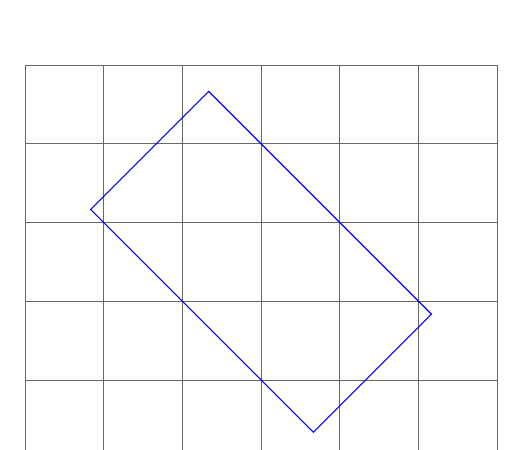
\begin{tikzpicture}[
  blocked/.style={rectangle,draw=black!60,fill=black!50,minimum size=0.5cm}
]

\draw[step=1cm,black!60,very thin,xshift=-0.5cm,yshift=-0.5cm] (0,0) grid (6,5);

\begin{scope}[xshift=2.5cm,yshift=2cm]
\draw [color=blue,rotate=45] (-1.06,-2) rectangle (1.06,2);
\end{scope}

\end{tikzpicture}

\end{itemize}

\section{TODO}

Things to fix in the implementation:
\begin{itemize}
 \item Enforce range constraints.
 \item Remove (or specify) support for \texttt{CheckFoundation} of \texttt{Unit} shapes.
 \item Fix \texttt{CheckBuildingPlacement} to skip shapes, and put foundations in the navcell grid.
 \item Support dynamic updates.
 \item Remove cost class parameters.
 \item Fix vector pathfinder to not do quadrant stuff.
 \item Set up passability classes for the current units.
 \item Testing.
 \item Fix the navcell grid vectorisation.
 \item Don't use long pathfinder for min range movement.
 \item AI integration.
 \item Make impassable-navcell-escaping work properly.
 \item A* heuristic overestimate with large goals.
 \item ...
\end{itemize}

\end{document}
